\chapter{Artigo: Ambient noise tomography across Parnaíba Basin}

Essa seção corresponde a terceira etapa do projeto, a qual consiste em  calcular as velocidades de propagação das ondas de superfície através da correlação do ruído sísmico ambiental e procurar um modelo que melhor se ajuste às anomalias de velocidades encontradas. Nesta parte do trabalho iremos utilizar um banco de dados maior, envolvendo estações de 4 redes sismográficas diferentes. Esse banco de dados consiste de um total de 31 estações de banda larga provenientes das redes RSBR (Rede Sismográfica Brasileira), RSISNE (Rede Sismográfica do Nordeste do Brasil), BODES (estações instaladas entre 2014 e 2016 numa transecta N-S na Provincia Borborema) e BP (rede utilizada nas estapas anteriores). Uma feição interessante que será o foco nessa etapa é o Lineamento Transbrasiliano,  descontinuidade de magnitude continental situada entre o Cráton Amazônico e a porção leste da Plataforma Sul-Americana. O objetivo principal desse trabalho é imagear essa mega-estrutura dentro da bacia, pois a subsidência e a deposição estão fortemente ligadas a essa estrutura \citep{vaz_bacia_2007}.

\begin{figure}[!ht]
\begin{center}
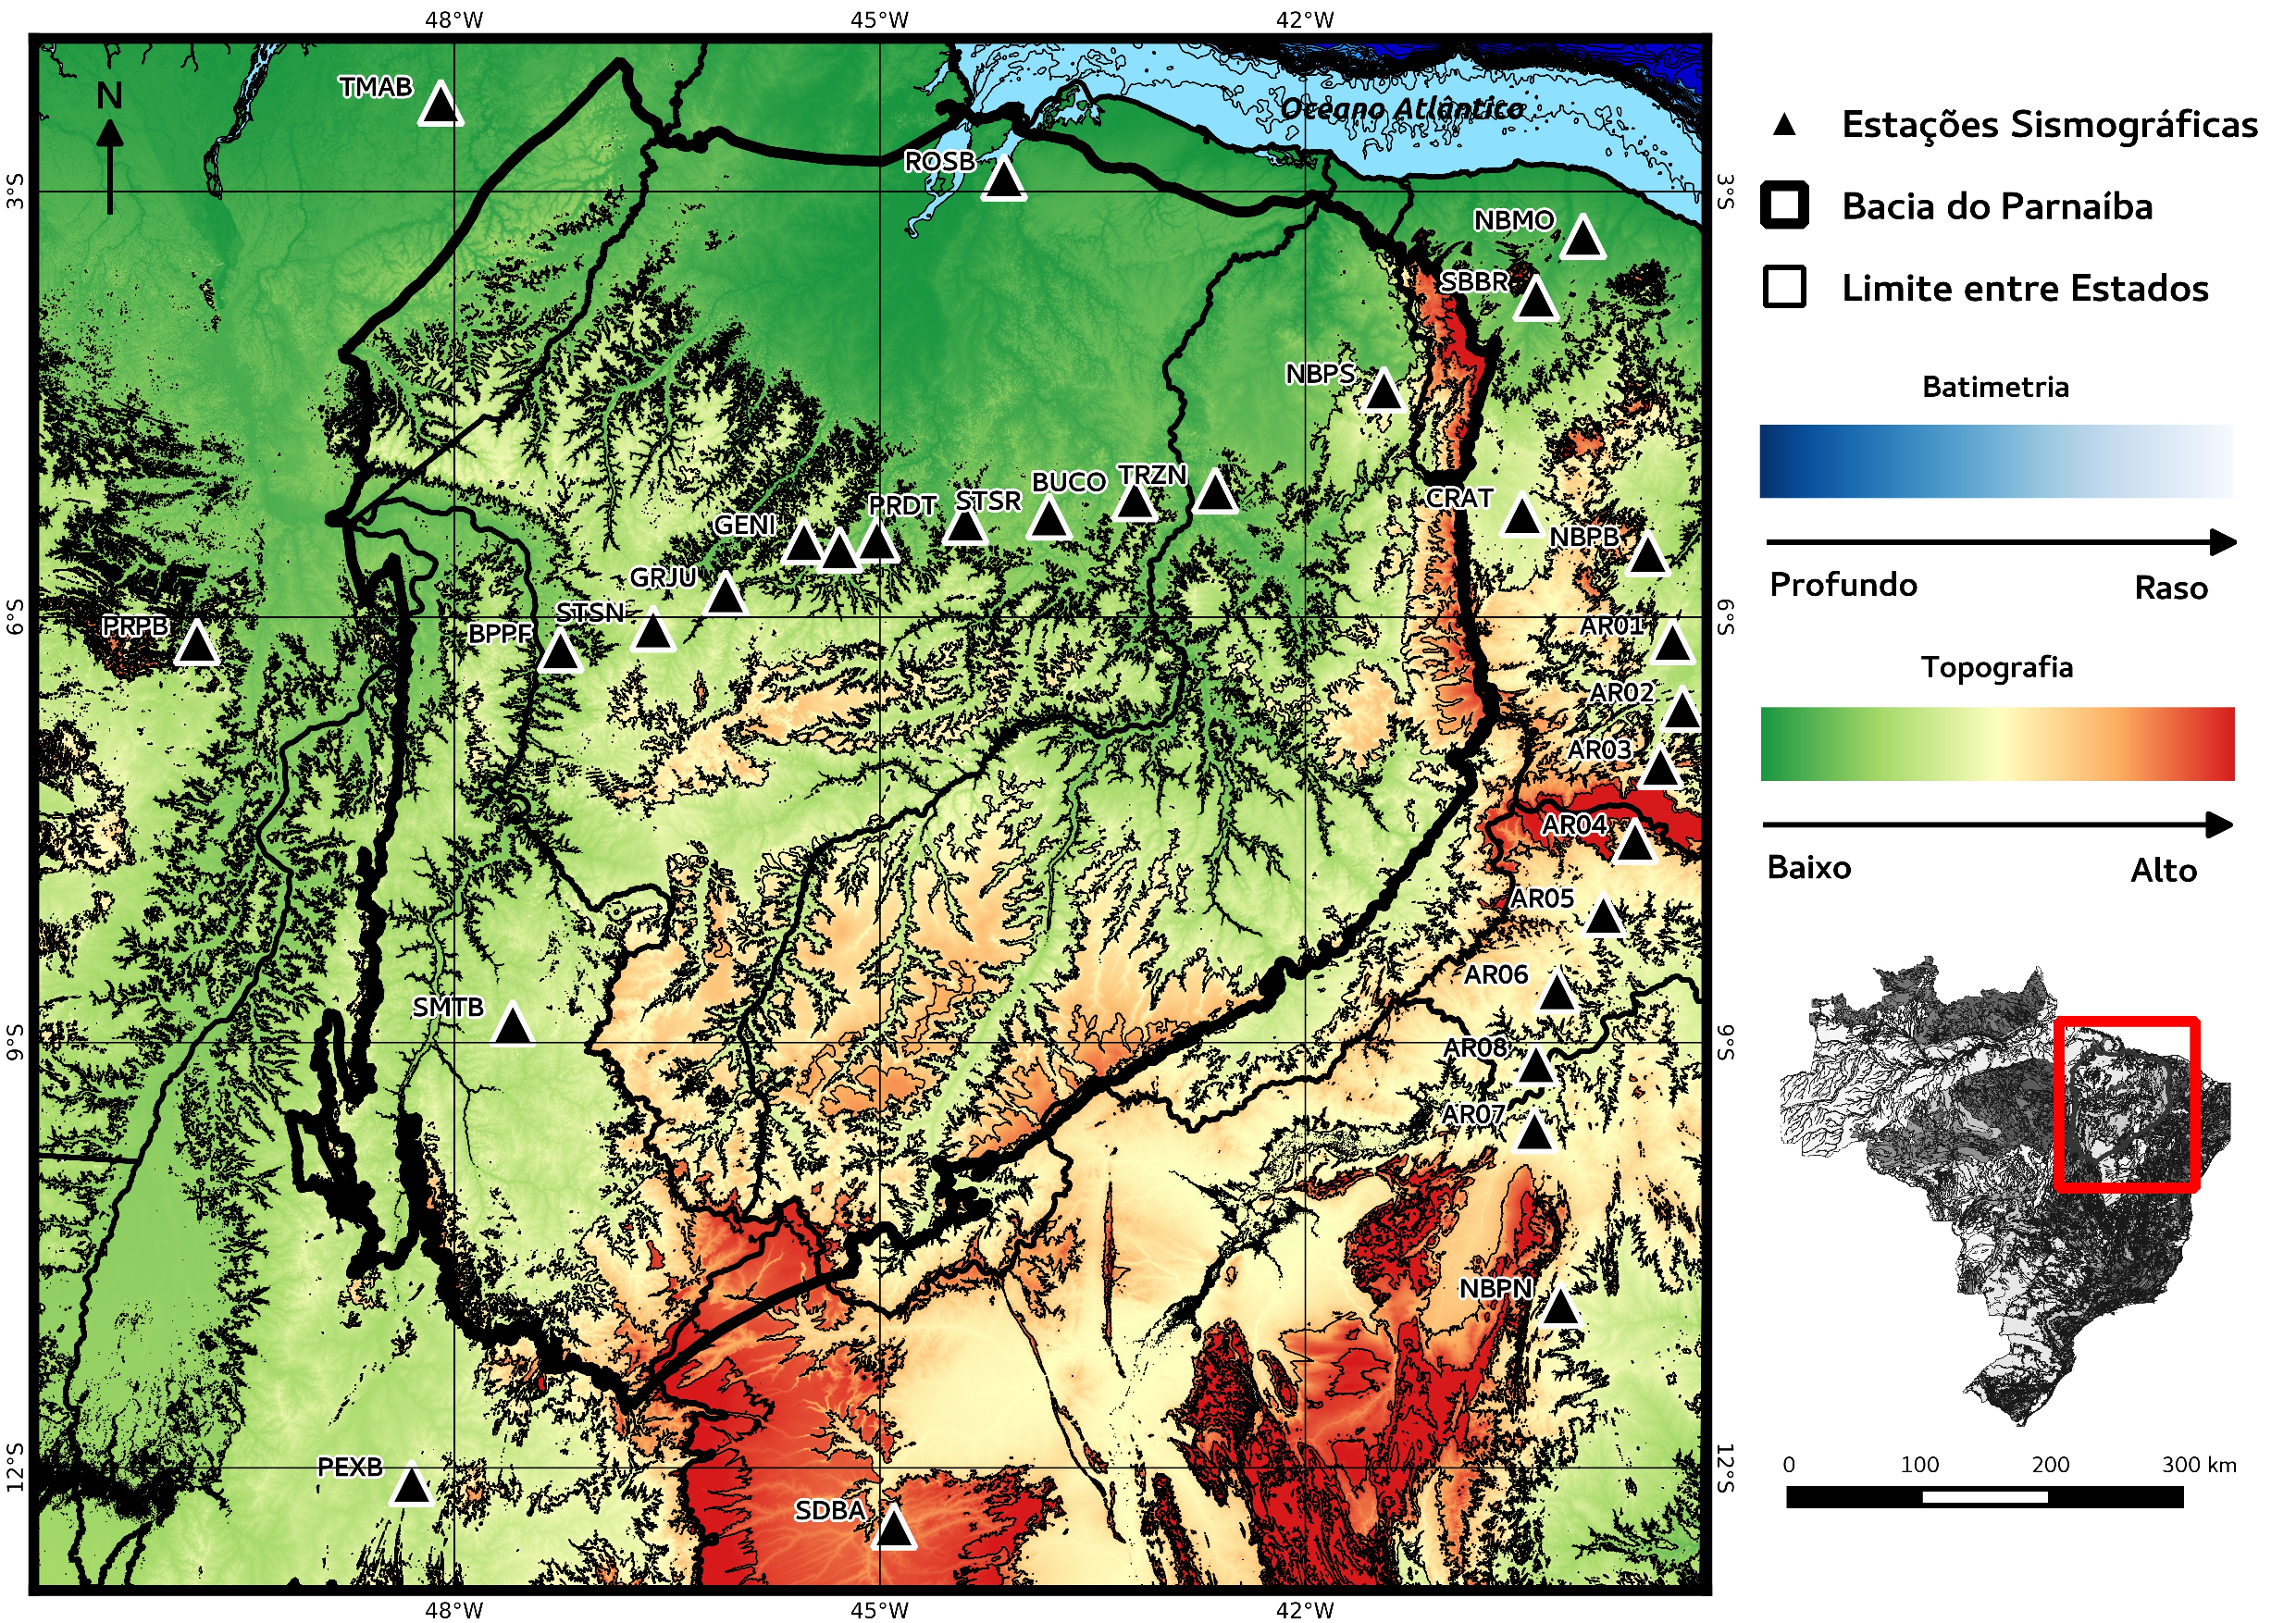
\includegraphics[width=1\textwidth]{Fig/mapa_topografico_estacoes_ambient_noise_BB.pdf}
\caption{Mapa com as estações da rede da BP, BODES, RSISNE e RSBR na Bacia do Parnaíba e na sua vizinhança.}
\label{mapa_sta_ambient_noise}
\end{center}
\end{figure}